\documentclass[tikz]{standalone}

\usepackage{fontspec}
\setmainfont[Ligatures=TeX, Mapping=tex-text]{Lato}
\setmonofont{FreeMonoBold}
\usepackage{tikz}
\usetikzlibrary{arrows.meta}
\usepackage{xfp}

\begin{document}
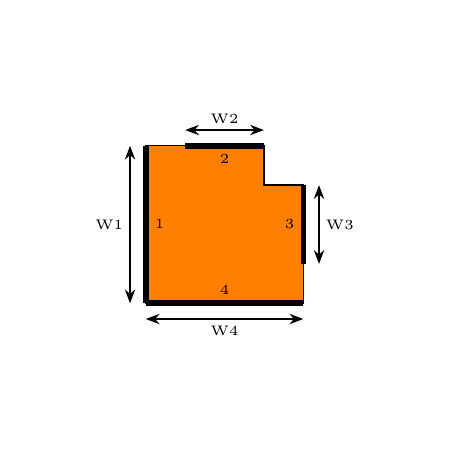
\begin{tikzpicture}

\def\width{5}
\def\height{5}
\def\ox{\fpeval{\width /2}}
\def\oy{\fpeval{\height /2}}

\tiny
\path [use as bounding box] (0,0) rectangle (\width,\height);

% SHAPE
\filldraw [line width=0.5pt, fill=orange] (\ox,\oy)
	+(-1,-1) --
	+(1,-1) --
	+(1,0.5) --
	+(0.5,0.5) --
	+(0.5,1) --
	+(-1,1) --
	cycle;

% PORTS
\draw [line width=2pt] (\ox,\oy) ++(-1,0) node[right] {1} +(0,-1) -- +(0,1);
\draw [line width=2pt] (\ox,\oy) ++(0,1) node[below] {2} +(-0.5,0) -- +(0.5,0);
\draw [line width=2pt] (\ox,\oy) ++(1,0) node[left] {3} +(0,-0.5) -- +(0,0.5);
\draw [line width=2pt] (\ox,\oy) ++(0,-1) node[above] {4} +(-1,0) -- +(1,0);

% DIMENSIONS
\draw [line width=0.5pt, {Stealth[length=5pt]}-{Stealth[length=5pt]}]
	(\ox,\oy) ++(-1.2,0) node[left] {W1}
	+(0,-1) -- +(0,1);
\draw [line width=0.5pt, {Stealth[length=5pt]}-{Stealth[length=5pt]}]
	(\ox,\oy) ++(0,1.2) node[above] {W2}
	+(-0.5,0) -- +(0.5,0);
\draw [line width=0.5pt, {Stealth[length=5pt]}-{Stealth[length=5pt]}]
	(\ox,\oy) ++(1.2,0) node[right] {W3}
	+(0,-0.5) -- +(0,0.5);
\draw [line width=0.5pt, {Stealth[length=5pt]}-{Stealth[length=5pt]}]
	(\ox,\oy) ++(0,-1.2) node[below] {W4}
	+(-1,0) -- +(1,0);

\end{tikzpicture}
\end{document}
